Esitellään mitä tarkoitetaan hajautetulla järjestelmällä (SOA) ja esitellään hajautettuihin järjestelmiin suunniteltuja protokollia, aikajärjestyksessä  kerberos -> saml -> oauth ja päädytään oauthiin, tarkemmin versioon 2.

Tunnistautumiseen liittyvien käsitteiden läpikäynti ennen protokollien yksityiskohtaista esittelyä auttaa tunnistautumiseen liittyvien periaatteiden hahmottamista. Käsitteet ovat yleisluontoisia ja eivätkä kosketa vain tiettyjä protokollaa. Protokollien yhteydessä käytetään käsitteitä asiakasohjelma, tunnistautumispalvelu, suojattu resurssi, valtuutustieto (credentials), valtuutusavain (authorization code) ja pääsyvaltuutus (access token) \cite{nisti}.

Asiakasohjelmalla tarkoitetaan web-palvelun käyttäjän pääteohjelmaa, jolla hän kirjautuu web-palveluun käyttäen keskitettyä tunnistautumispalvelua. Käytännössä asiakasohjelma on web-palvelun tapauksessa käyttäjän WWW-selain, joka pystyy tekemään uudelleenohjauksia sivustolta toiselle. Uudelleenohjaus on HTTP-protokollan perustoiminnallisuutta, joten mikä tahansa HTTP/1.1-standardin WWW-selain käy asiakasohjelmaksi \cite{rfc2616}.

Tunnistautumispalvelu on web-palvelu, johon käyttäjä ohjataan tekemään tunnistautuminen. Onnistuneen tunnistautumisen jälkeen tunnistautumispalvelu ohjaa asi\-a\-kas\-oh\-jel\-man takaisin tunnistautumista pyytäneen palvelun määrittelemään osoitteeseen \cite{nisti}. Avoimen Internetin puolella tunnistautumispalvelu voi olla esimerkiksi Facebook tai LinkedIn.

Tunnistautumisprotokollien yhteydessä suojatulla resurssilla tarkoitetaan resurssia, jonka käyttö vaatii tunnistautumisen ja käyttöoikeuden. Yleisessä tapauksessa suojatulla resurssilla tarkoitetaan yksittäistä resurssia (käyttäjän valokuvaa), johon halutaan asettaa pääsyrajoituksia \cite{nisti}. Tämän tutkielman puitteissa suojatulla resurssilla tarkoitetaan tunnistautumista vaativaa web-palvelua.

Valtuutustieto koostuu yksilöivästä tunnisteesta ja siihen liittyvästä salaisesta avaimesta. Tämän tutkielman puitteissa valtuutustiedolla tarkoitetaan käyttäjän tunnusta ja salasanaa.

Kirjauduttuaan sisään tunnistautumispalvelimelle, käyttäjä saa valtuutusavaimen, jonka hän lähettää eteenpäin suojatun resurssin omistajalle. Valtuutusavain ei pidä sisällään käyttäjän valtuutustietoja, vaan ainoastaan tunnistautumispalvelin osaa lukea sen \cite{nisti}. Saatuaan valtuutusavaimen käyttäjältä voi suojatun resurssin omistaja hakea pääsyvaltuuden käyttäjän tietoihin tunnistautumispalvelusta.

Pääsyvaltuutus on tunnistautumispalvelimelta saatava yksilöivä tunniste, jonka avulla suojatun resurssin omistaja voi pyytää käyttäjän tiedot tunnistautumispalvelulta. Pääsyvaltuutus on voimassa tietyn ajan, jonka jälkeen se täytyy uusia tunnistautumispalvelimella \cite{nisti}. Pääsyvaltuutusta voidaan käyttää myös tunnistautumispalvelusta erillään olevien resurssien valtuuttamiseen. Esimerkiksi web-sovellus voi hakea tunnistautumispalvelulta pääsyvaltuuden, jolla hän hakee valokuvia valokuvien jakopalvelusta \cite{facebook}.
\subsection{Ongelmakenttä}
Palvelusuuntauneissa web-ohjelmistoissa käyttäjien tunnistautuminen on toteutettu monin tavoin. Tyypillisesti kysytään käyttäjältä tunnus ja salasana, joita verrataan ohjelmiston paikalliseen käyttäjätietokantaan. Paikallinen tietokanta on kopioitu palvelun varsinaisesta käyttäjätietokannasta ja paikallisiin tietokantoihin on käyttäjille luotu erillinen käyttäjätunnus.

Tästä seuraa monenlaisia synkronointiongelmia. Esimerkiksi työntekijän irtisanoutuessa joudutaan tunnus poistamaan kaikista tietokannoista erikseen. Myös osoitteen yms. tietojen muutokset täytyy päivittää kaikkiin tietokantoihin. Lisäksi käyttäjälle syntyy saman järjestelmän sisällä monia tunnuksia, joihin saattaa liittyä erilliset salasanat. Käyttäjän kannalta on myöskin ikävää kirjautua jokaiseen osapalveluun erikseen.
\subsection{Ympäristö}
Lähteet:\\
- inside the identity management game \cite{inside_the_identity_management_game}\\
- Decentralization: The Future of Online Social Networking \cite{decentralisations}

Tyypillisesti web-palvelun toimintakenttä on Internet, jossa palvelut toimivat itsenäisesti. Näiden palveluiden välinen integraatio on kasvussa ja palveluiden kesken halutaan jakaa tietoa, jolloin niiden täytyy pystyä identifioimaan käyttäjä keskenään. Yleisen identeettitarjoajan rakentaminen Internettiin on tutkimuksen alla ja OpenID ja mitä näitä nyt on. 

Usein ei ole tarpeen tehdä palveluista julkisia, vaan käyttöoikeus niihin voidaan rajata tietylle osajoukolle kaikista Internetin käyttäjistä. Tällaisia osajoukkoja voi olla esimerkiksi yrityksen työntekijät, joilla on pääsy intranet-palveluihin tai tietyn sivuston käyttäjät, joilla on pääsy sivuston palveluihin. Tällöin voi olla järkevää eriyttää käyttäjähallinta omaksi palveluksi ja keskittää osapalveluiden tunnistautuminen siihen. Tämän tutkielman pääpaino on tunnetulle osajoukolle, esimerkiksi yrityksen työntekijöille, suunnatuissa palveluissa.

Tutkielmassa pyritään selvittämään kuinka yritys voi rakentaa keskitetyn tunnistautumispalvelun valmiin käyttäjädatan päälle. Lähtökohtaisesti tunnistautumista vaativat palvelut ovat web-pohjaisia, mutta myös työasemalla tai puhelimella käytettävät asiakasohjelmat pyritään ottamaan huomioon.

\subsection{Tunnistaumisen periaatteet}
Keskitetyn tunnistautumisen lähtökohta on käyttäjän tunnistetietojen poistaminen web-palvelun hallinnasta. Käyttäjä ei syötä tunnistetietojaan missään vaiheessa web-palveluun, vaan tunnistautuminen tehdään erillisessä tunnistautumispalvelussa. Nykyisin mm. Facebook ja Google tarjoavat julkiset API-rajapinnat, joiden avulla web-palvelut voivat käyttää niitä tunnistautumiseen \cite{facebook}.

Facebook-kirjautuminen on käytössä monissa web-palveluissa ja sen käyttö on suoraviivaista. Kuvassa \ref{facebook_login} on kuvattu kirjautuminen Porkkanamafia-ryhmän WWW-sivulle käyttäen Facebookia. Käyttäjä klikkaa WWW-sivulla olevaa ''Login with Facebook'' -nappia, jonka jälkeen käyttäjän selaimeen avautuu Facebookin varmennusikkuna, jossa käyttäjää pyydetään varmentamaan kirjautuminen. Selaimen osoitekenttä osoittaa käyttäjälle, että kirjautuminen tapahtuu nimenomaan Facebook-sivulla (joka on varmennettu SSL-sertifikaatilla), joten käyttäjän Facebook-tun\-nis\-te\-tie\-dot eivät päädy Porkkanamafian haltuun, vaan kirjautuminen hoidetaan suoraan Facebookiin \cite{facebook}.

Kirjautumisen jälkeen käyttäjälle luodaan rivi käyttäjätietokantaan, jossa on viittaus hänen Facebook-tunnukseensa. Kun käyttäjä tämän jälkeen palaa sivulle ja kirjautuu sisään jälleen Facebook-tunnuksilla, voidaan käyttäjä yhdistää kannasta löytyvään vanhaan käyttäjään. Näin palvelu on ulkoistanut tunnistautumisen ulkopuoliselle taholle, eikä käyttäjän tarvitse muistaa uusia tunnistetietoja, vaan hän voi käyttää Facebook-kirjautumista jatkossa tullessaan Porkkanamafian sivulle.

Samaa periaatetta voidaan käyttää myös organisaatioiden sisäisessä tunnistautumispalvelussa. Organisaation sisäiseen palvelusuuntautuneeseen arkkitehtuuriin toteutetaan erillinen web-palvelu, joka on yhteydessä olemassa olevaan käyttäjätietokantaan (esim. LDAP) ja tarjoaa Facebookia vastaavan tunnistautumisen.

\begin{figure}[ht]
\centering
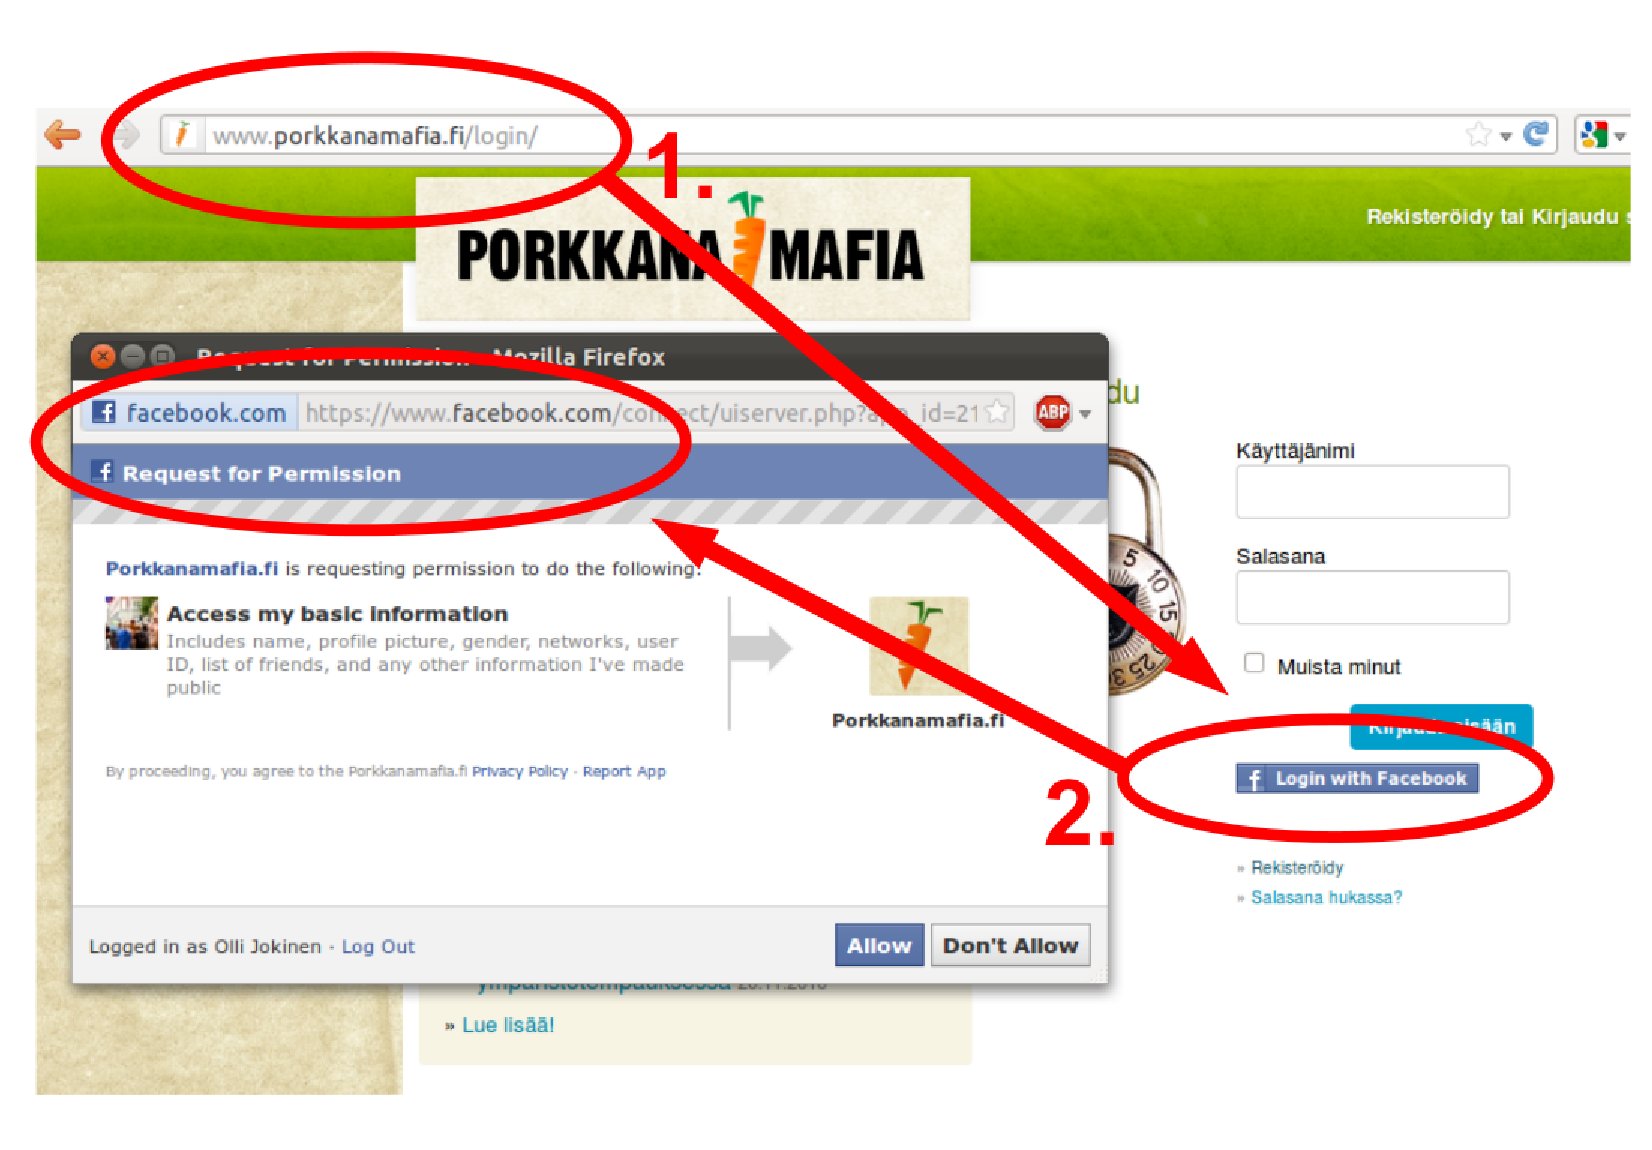
\includegraphics[width=0.7\textwidth]{teknologiat/facebook.eps}
\caption{Käyttäjän kirjautuminen Facebook-tunnuksilla Porkkanamafian web-palveluun.}%
\label{facebook_login}
\end{figure}
\subsection{Tunnistautumisen rajapintaprotokollat}
Tunnistautumiseen liittyvien käsitteiden läpikäynti ennen protokollien yksityiskohtaista esittelyä auttaa tunnistautumiseen liittyvien periaatteiden hahmottamista. Käsitteet ovat yleisluontoisia ja eivätkä kosketa vain tiettyjä protokollaa. Protokollien yhteydessä käytetään käsitteitä asiakasohjelma, tunnistautumispalvelu, suojattu resurssi, valtuutustieto (credentials), valtuutusavain (authorization code) ja pääsyvaltuutus (access token) \cite{nisti}.

Asiakasohjelmalla tarkoitetaan web-palvelun käyttäjän pääteohjelmaa, jolla hän kirjautuu web-palveluun käyttäen keskitettyä tunnistautumispalvelua. Käytännössä asiakasohjelma on web-palvelun tapauksessa käyttäjän WWW-selain, joka pystyy tekemään uudelleenohjauksia sivustolta toiselle. Uudelleenohjaus on HTTP-protokollan perustoiminnallisuutta, joten mikä tahansa HTTP/1.1-standardin WWW-selain käy asiakasohjelmaksi \cite{rfc2616}.

Tunnistautumispalvelu on web-palvelu, johon käyttäjä ohjataan tekemään tunnistautuminen. Onnistuneen tunnistautumisen jälkeen tunnistautumispalvelu ohjaa asi\-a\-kas\-oh\-jel\-man takaisin tunnistautumista pyytäneen palvelun määrittelemään osoitteeseen \cite{nisti}. Avoimen Internetin puolella tunnistautumispalvelu voi olla esimerkiksi Facebook tai LinkedIn.

Tunnistautumisprotokollien yhteydessä suojatulla resurssilla tarkoitetaan resurssia, jonka käyttö vaatii tunnistautumisen ja käyttöoikeuden. Yleisessä tapauksessa suojatulla resurssilla tarkoitetaan yksittäistä resurssia (käyttäjän valokuvaa), johon halutaan asettaa pääsyrajoituksia \cite{nisti}. Tämän tutkielman puitteissa suojatulla resurssilla tarkoitetaan tunnistautumista vaativaa web-palvelua.

Valtuutustieto koostuu yksilöivästä tunnisteesta ja siihen liittyvästä salaisesta avaimesta. Tämän tutkielman puitteissa valtuutustiedolla tarkoitetaan käyttäjän tunnusta ja salasanaa.

Kirjauduttuaan sisään tunnistautumispalvelimelle, käyttäjä saa valtuutusavaimen, jonka hän lähettää eteenpäin suojatun resurssin omistajalle. Valtuutusavain ei pidä sisällään käyttäjän valtuutustietoja, vaan ainoastaan tunnistautumispalvelin osaa lukea sen \cite{nisti}. Saatuaan valtuutusavaimen käyttäjältä voi suojatun resurssin omistaja hakea pääsyvaltuuden käyttäjän tietoihin tunnistautumispalvelusta.

Pääsyvaltuutus on tunnistautumispalvelimelta saatava yksilöivä tunniste, jonka avulla suojatun resurssin omistaja voi pyytää käyttäjän tiedot tunnistautumispalvelulta. Pääsyvaltuutus on voimassa tietyn ajan, jonka jälkeen se täytyy uusia tunnistautumispalvelimella \cite{nisti}. Pääsyvaltuutusta voidaan käyttää myös tunnistautumispalvelusta erillään olevien resurssien valtuuttamiseen. Esimerkiksi web-sovellus voi hakea tunnistautumispalvelulta pääsyvaltuuden, jolla hän hakee valokuvia valokuvien jakopalvelusta \cite{facebook}.
\subsubsection{Kerberos}
Lähteet:
Enhancing Distributed Web Security Based on Kerberos Authentication Service
Secure Secret-Key Management of Kerberos Service

Kerberos-protokolla on alunperin MIT:ssa kehitetty tunnistautumisprotokolla, jonka nykyisin käytössä oleva versio 5 julkaistiin alunperin syyskuussa 1993 ja päivitettynä heinäkuussa 2005 [RFC4120]. Se on yleisesti käytössä erilaisissa UNIX-pohjaisissa käyttöjärjestelmissä ja myös Microsoft on käyttänyt sitä oletus-tunnistautumismekanismina Windows 2000:sta lähtien [RFC3244].

Protokollan osapuolia ovat käyttäjä, luotettava kolmas osapuoli ja palvelu, joka vaatii tunnistautumisen. Luotettava kolmas osapuoli on tyypillisesti avaintenjakopalvelin (KDC, Key Distribution Center), joka tunnistaa käyttäjän ja myöntää lipun tunnistautuneelle käyttäjälle. Myönnettyyn lippuun on merkattu palvelu, johon sitä voidaan käyttää ja aikaleima, jonka ajan se on voimassa. Käyttäjä antaa lipun tunnistautumista vaativalle palvelimelle, joka tarkistaa omalla avaimellaan käyttäjän tunnisteen ja aikaleiman, joiden perusteella se myöntää pääsyn palveluun.

Keskitetty tunnistautuminen hajautettuihin järjestelmiin voidaan toteuttaa Kerberos-protokollalla [Enhancing...]. Kerberos on luonteeltaan sopiva hajautettuihin järjestelmiin, koska avaintenjakopalvelin voi jakaa lippuja kaikkiin järjestelmiin, joiden kanssa se on vaihtanut salausavaimet. Tunnistautumispalvelin on tilaton, jolloin sen suorituskykyä voidaan parantaa tarvittaessa skaalaamalla, joten tunnistautumispalvelin voi palvella suurta määrää käyttäjiä [Enhancing...].

Tunnistautumisessa käytetyt yksityiset avaimet tallennetaan tietokantaan, jolloin on riskinä, että kolmas osapuoli saattaa päästä käsiksi näihin avaimiin ja pystyä allekirjoittamaan lippuja. Jakamalla salaiset avaimet osiin ja hajauttaa se avaintenjakopalvelimeen, tunnistautumista vaativalle palvelimelle ja näiden välillä käytetylle reitittimelle [Secure Secret-Key...], voidaan parantaa protokollan luotettavuutta. Tämä tekee siitä mahdollisen vaihtoehdon käytetyksi menetelmäksi keskitettyyn tunnistautumiseen hajautetuissa järjestelmistä.

\subsubsection{SAML}
Security Assertion Markup Language (SAML) on OASIS-komitean määrittelemä XML-pohjainen avoin standardi tunnistautumiseen ja pääsynhallintaan \cite{saml_spec}. Standardin versio 1.0 julkaistiin marraskuussa 2002 ja versio 2.0 maaliskuussa 2005. Version 2.0:n viimeisin korjattu versio 5 julkaistiin helmikuussa 2012.

SAML määrittelee XML-pohjaiset työkalut tunnistautumisen ja pääsynhallinnan toteuttamiseen. Varsinainen toteutus, esimerkiksi se, mitä tietoja siirretään ja millä tavalla, jätetään SAML:ssä toteuttajan päätettäväksi \cite{dynamic_saml}. Varsinaiset SAML-viestit voivat kulkea esimerkiksi synkronisesti SOAP- ja HTTP-protokollalla. SAML soveltuu avoimena ja XML-pohjaisena protokollana käytettäväksi Web Services -standardilla toteutetuissa web-sovelluksissa.

Standardi koostuu useista eri komponenteista, jotka yhdessä muodostavat SAML v2.0 -spesifikaation \cite{saml_spec}. Keskeisempänä ovat vakuutukset (assertion), joihin sovellukset voivat luottaa. Nämä vakuutukset koskevat tunnistautumista, pääsynvalvontaa sekä attribuutteja. SAML:ssa on määritelty myös protokollasidokset (protocol bindings), joiden mukaan vakuutukset siirtyvät järjestelmästä toiseen. Yhdessä nämä muodostavat profiileja, joiden avulla esimerkiksi keskitetty tunnistautuminen voidaan toteuttaa \cite{saml_spec}.

SAML on vakiintunut standardi ja siihen on määritelty erilaisia laajennoksia, joiden ansiosta samalla standardilla voidaan toteuttaa koko identiteentinhallinta \cite{saml_spec}. Tästä syystä se on vakiintunut standardina erityisesti yritysten sisäisissä kertakirjautumisratkaisuissa (Single Sign On) \cite{dynamic_saml}. Kuitenkaan niin kutsutun julkisen Internetin puolella SAML ei ole saavuttanut merkittävää asemaa, vaan yritykset kuten Google ja Facebook ovat toteuttaneet omat tunnistautumisrajapintansa kevyemmillä protokollilla, kuten OpenID:llä ja OAuthilla.
\subsubsection{OAuth}
Tämä kappale tulee luultavasti muuttumaan, yleisiä juttuja johdantoon ja tähän vain Oauth-spesifistä asiaa, miten eroaa kerberoksesta jne. Pituus 2-3 sivua, kuvia yms. Oleellisin näistä protokollista, koska tullaan käyttämään toteutuksessa.

OAuth on avoin tunnistautumisrajapinta hajautetuille web-sovelluksille. Se mahdollistaa käyttäjien resurssien jakamisen palveluiden välillä ilman käyttäjätunnuksen tai salasanan luovuttamista kolmannelle osapuolelle. Se perustuu erilaisten valtuutusavainten (token) välittämiseen palveluiden välillä. OAuth on yleisesti käytössä web-sovelluksissa, joissa halutaan näyttää käyttäjälle kuuluvia resursseja (esimerkiksi valokuvia), jotka sijaitsevat toisessa sovelluksessa [TODO: lähde].

OAuth on määritelty RFC-dokumentissa numero 5849. Sen ensimmäinen versio (1.0) julkaistiin lokakuussa 2007 ja päivitetty versio (1.0a) kesäkuussa 2009 \cite{oauth2_0}. OAuthin versio 2.0 on myös kehitteillä ja se on tarkoitus julkaista marraskuussa 2012 \cite{oauth2_0}.

Alunperin OAuthin kehitystyö alkoi marraskuussa 2006, kun Blaine Cook kehitty Twitter-palveluun OpenID-tukea.

... tarvitaanko tätä?

\begin{figure}[ht]
\centering
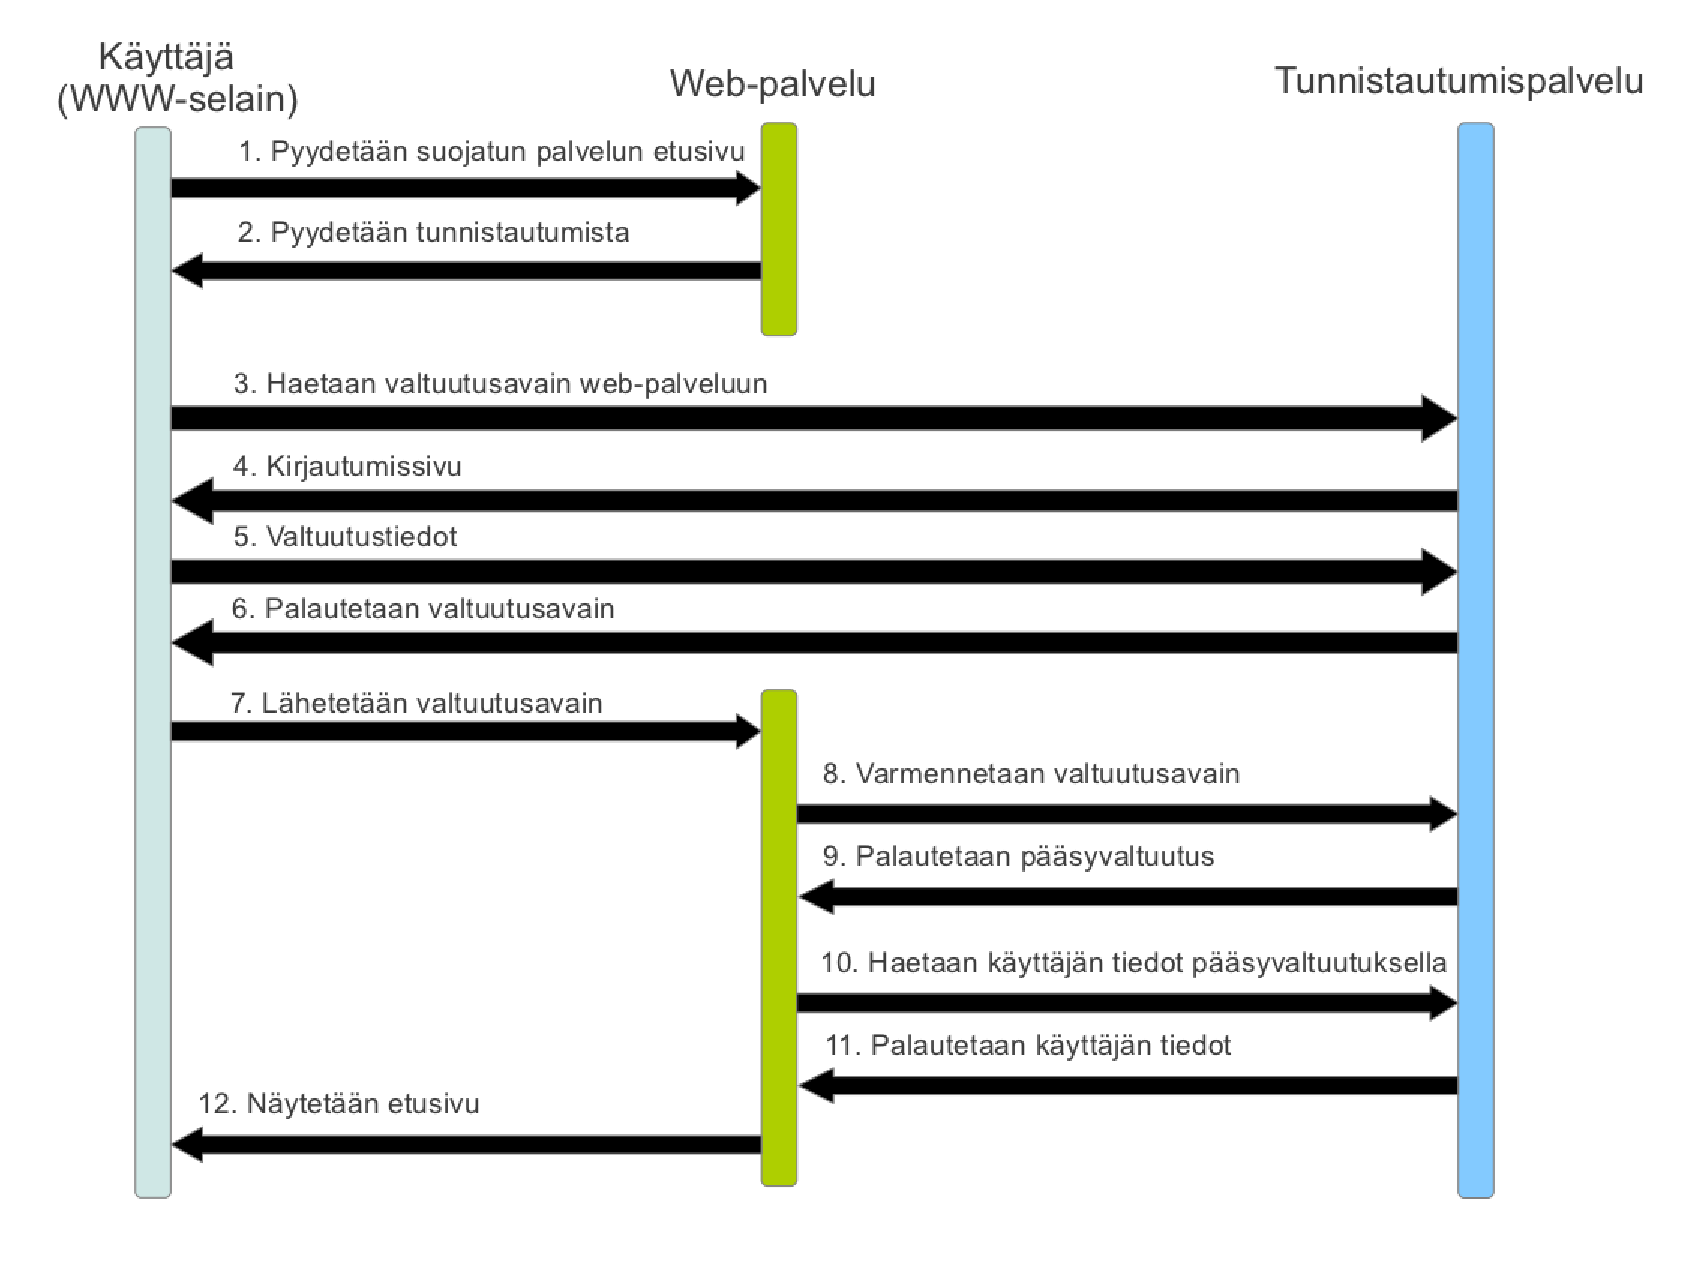
\includegraphics[width=\textwidth]{teknologiat/protokollat/oauth.eps}
\caption{OAuth sekvenssikaavio}%
\label{oauth}
\end{figure}

\subsection{Yhteenveto}
Käytetään OAuthia protossa, koska OpenID:ssä kaikkea tarpeetonta mukana. SAML taas skipataan, koska...? Tätä pitäisi pohtia jossain kohtaa.